\documentclass{beamer}
\usepackage[utf8]{inputenc}
\usetheme{Warsaw}
\title{Présentation Tâche 5:\\ dimensionnement d'une soupape de sécurité}
\author{Groupe 1246}
\institute{École Polytechnique de Louvain}
\date{}
\begin{document}

\begin{frame}
\titlepage
\end{frame}

\begin{frame}{Démarche}
\begin{figure}[ht!]
\centering
\includegraphics[scale=0.4]{demarche.PNG}
\end{figure}
\end{frame}

\begin{frame}
\frametitle{Dimensionnement de la soupape}
\begin{itemize}
\item aire donnée par:$$A=\dfrac{W}{CK_dP_1K_bK_c}\cdot \sqrt{\dfrac{TZ}{M}}$$
\item $W$ est le flux massique en $\left[ \dfrac{Kg}{h}\right] $
\item $K_d$,$K_b$, $Z$ et $K_c$ sont des constantes connues
\item $P_1$ est la pression de design  + surpression + 1atm (en $\left[ kPa \right]$ )
\item $T$ est la temperature en $[K]$
\item $M$ est la masse molaire du composé
\item $C$ est un coefficient à déterminer
\end{itemize}
\end{frame}

\begin{frame}{Dimensionnement de la soupape}
\framesubtitle{Pression $P_1$ vs Temperature T}
\begin{figure}[ht!]
\centering
\includegraphics[scale=0.5]{graph3.PNG}
\end{figure}
\end{frame}

\begin{frame}
\frametitle{Dimensionnement de la soupape}
\framesubtitle{Calcul de $C$ et $W$}
$$C=0.03948\sqrt{k\left( \dfrac{2}{k+1}\right)^{\left( \dfrac{k+1}{k-1}\right)}}$$
\begin{itemize}
\item où $k$ est le raport $\dfrac{C_p}{C_v}$
\end{itemize}
$$W=\dfrac{Q}{\Delta H_{vap}}$$
\begin{itemize}
\item avec $Q=C_1FA_{ws}^{0.82}$
\begin{itemize}
\item $C_1$ est constante
\item $F$ est un facteur environnemental
\item $A_{ws}$ est la surface mouillée
\end{itemize}
\end{itemize}
\end{frame}

\begin{frame}{Dimensionnement de la soupape}
\framesubtitle{Facteur environemental}
\begin{figure}[ht!]
\centering
\includegraphics[scale=0.5]{facteur.PNG}
\end{figure}
le facteur environnemental est différent en fonction du type de stockage.
\end{frame}

\begin{frame}{Dimensionnement de la soupape}
\framesubtitle{Modèle standard de soupape}
\begin{figure}[ht!]
\centering
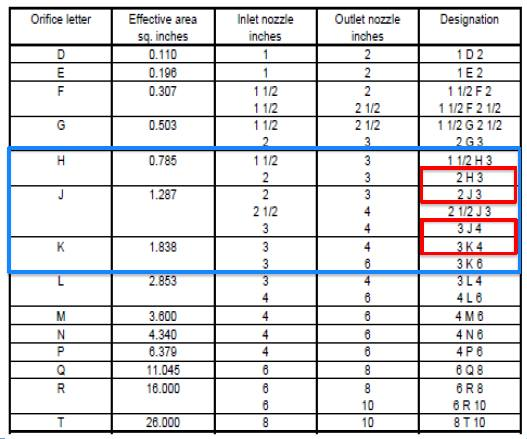
\includegraphics[scale=0.5]{tab.PNG}
\end{figure}
Modèles de soupapes en fonction de la taille de l'orifice calculé.
\end{frame}
\end{document}
